\ifx\wholebook\relax\else
\input{../Common.tex}
\input{../macroes.tex}
\begin{document}
\fi


\chapter{Strings and Tools to Understand Programs}\label{ch:strings}

In this chapter I present an important concept: the notion of strings. 
A string is a sequence of characters that represents words or sentences. Strings
are used to communicate with users. We shall use strings in the subsequent chapters as a tool to help you understand condition and conditional loops. In this chapter I limit myself to the most important aspects of strings and present the minimal information that you will use in subsequent chapters. I also present how you can use strings to understand how programs are executed. Of course, I suggest you try to also use the debugger to understand the experiments I propose. 

\section{Strings}
Strings are used to represent information and present it to the user. Strings are delimited by single quotes (\ct{'}) and they can contain white space characters. For example, the following string \ct{'squeak is cool'} represents a sequence of 14 characters: s q u e a .... Note that a space in also a character. A string can contain any number of characters, even zero. \ct{''} is an empty string. \ct{'a'} is a string with only the character a. \ct{' '} is a string with only the character space. 

\cadre{A string is a sequence of characters delimited by  single quotes \ct{'}. A string  represent textual information such as words or sentences and is used to display information to the user.}


Selecting a string and printing it (menu print it) prints the same string.  Several methods are defined on strings: the most important one in the context of this book is the method \index{string concatenation} \ct{,} that given a string as receiver and one string as argument returns the concatenation of the two. It is for example possible to replace a string into another one using the method \ct{copyReplaceAll:} as shown below. 

\begin{nalltt}
'squeak'                                                      "the value of a string is itself"
\pr 'squeak'

'a'							"a string can be composed of only one character"

''                                                        "an empty string"

'squeak' , 'is cool'                                        "concatening two strings"
\pr 'squeakis cool'

'', 'squeak', ' ', 'is cool'                              "concatening multiple strings"
\pr 'squeak is cool'

'Squeak is not cool' copyReplaceAll: 'not' with: 'really' 
\pr	'Squeak is really cool'
\end{nalltt}


\section{Communicating with the User}

Squeak offers some tools to display and request information. The \ct{PopUpMenu} allows one to bring up a menu and to display some sentences. For example, the expression \ct{PopUpMenu inform: 'squeak is cool'} pop ups a small window displaying the message 'squeak is cool' and waits that the user presses the ok button. 
\ct{FillInTheBlank} allows you to request some input from the user. For example the expression \ct{FillInTheBlank request: 'is squeak cool?'} prompts a dialog box with an input field and waits that the user fills the input field and presses the accept button or simply the cancel button. The result of this expression is a string that represents the contents typed by the user. We can also specify a contents by default using the message \ct{request:initialAnswer:} as shown in the following script. 


\begin{minipage}[c]{0.5\linewidth}
\begin{nalltt}
PopUpMenu inform: 'squeak is cool'
\end{nalltt}
\end{minipage}
\begin{minipage}[c]{0.5\linewidth}
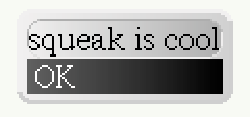
\includegraphics{inform}
\end{minipage}


\begin{minipage}[c]{0.5\linewidth}
\begin{nalltt}
FillInTheBlank request: 'is squeak cool?'  
\pr 'yes'

FillInTheBlank request: 'squeak cool?' initialAnswer: 'yes of course'
\pr 'yes'
\end{nalltt}
\end{minipage}
\begin{minipage}[c]{0.5\linewidth}
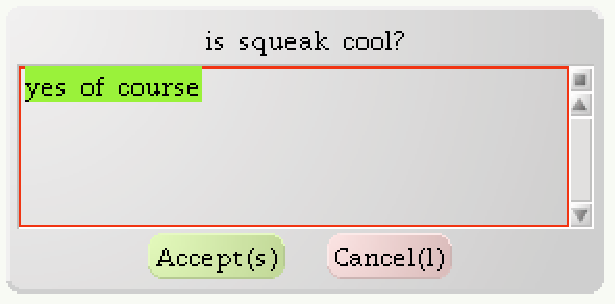
\includegraphics[width=.8\linewidth]{FillInTheBlank}
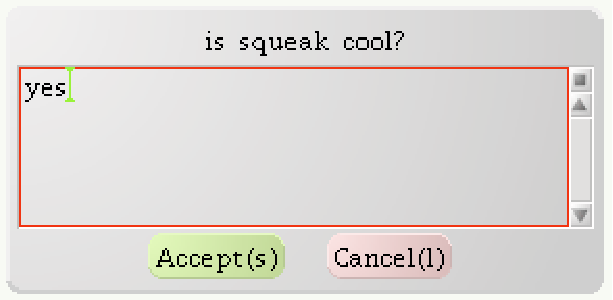
\includegraphics[width=.8\linewidth]{FillIn2}
\end{minipage}




\section{Strings and Characters}

A string is composed of characters. Individual characters are prefixed by a dollar sign \ct{\$}. For example, \ct{\$a} is character representing the letter \ct{a}.
Note that while individual characters are prefixed by the dollar sign \ct{\$}, when you edit a string we simply type characters without the dollar sign. 

Several methods allows one to access characters of strings. For example, the method \ct{first}, \ct{second}, \ct{third} return the first, second, and third characters of a strings. \ct{size} returns the string character number, \ct{at: aNumber} returns the character at the specified place, \ct{at: aNumber put: aCharacter} replaces the character at the position by a new character. The method \ct{copyUpTo: aCharacter} returns the beginning of a string up to the first character equals to aCharacter.


\begin{nalltt}
'squeak is cool' first 
\pr \$s

'squeak is cool' size
\pr 14

'squeak' at: 5
\pr \$a 

'squeak is cool' at: 11 put: $f
\pr 'squeak is fool'

'squeakiscool' copyUpTo: $i
\pr 'squeak'

'squeak is cool' copyUpTo: Character space
\pr 'squeak'
\end{nalltt}

To create character that do not have a graphical representation such as space, tab, carriage return, we simply send a message to the class \ct{Character}. The messages \ct{Character space}, \ct{Character tab}, and \ct{Character cr} return respectively the space, tab and carriage return character.

The following script~\ref{scr:atput} shows how we insert a carriage return inside a string. Note that the method \ct{at:put:} does not return the modified string but the character that was inserted. This is an example where the effect of the message and its results are clearly different. Printing the result of the message \ct{'squeak is cool' at: 7 put: Character cr} does not illustrate the effect of the method. Therefore we print the modified string.

\begin{scriptwithtitle}{Inserting a carriage return}\label{scr:atput}
|string|
string := 'squeak is cool'.
string at: 7 put: Character cr.
string \pr 'squeak
is cool'
\end{scriptwithtitle}

A character can also be converted into a string by sending it the message \ct{asString}.

\begin{scriptwithtitle}{}
'sque', $a asString, 'k'
\pr 'squeak'
\end{scriptwithtitle}

\section{Strings and Numbers}
A string can represent a number, for example the \emph{string} \ct{'10'} is a textual representation of the number 10. However, a string is not a number.  A string does not know out to perform any mathematical operation and a number does not know how to behave as a string. For example we cannot concatenate two numbers or add two strings. However, a number knows how to produce a string which represents it using the method \ct{asString}. In addition a string knows how to how to convert a representation of a number into a number using the method \ct{asNumber}. 


\cadre{A string can represent a number but this is not a number. For example, the string \ct{'69'} is composed of the two characters: \ct{\$6} and \ct{\$9}. To obtain the string representing a number, send the message \ct{asString} to it.}

There is a difference between the number \ct{10} and the string \ct{'10'}.  \ct{10} represents the mathematical number 10 while the string \ct{'10'} represents the number \ct{10}. The string \ct{'10'} is composed of two characters: \ct{\$1} and \ct{\$0}. The string \ct{'10'} is composed of two character \ct{\$1} followed by \ct{\$2}.

\begin{nalltt}
10 , 12 
-> error! a number does not know the message ,

'10', '12'
\pr '1012'

10 asString
\pr '10'

10 asString , 12 asString
\pr '1012'

'10' asNumber
\pr 10
\end{nalltt}


\section{Using the Transcript}
Squeak offers several powerful tools to understand program execution such as the debugger (see Chapter~\ref{ch:debugger}). Another tool is call the \ct{Transcript}. A transcript is a window in which you can display information given as strings. To open a transcript, drag into the desktop the thumbnail that is available in one of the flaps or you choose the \button{transcript} item of the \button{open...} menu entry. This opens a window as shown in Figure~\ref{fig:transcript}.

\begin{figure}[h]
\begin{center}
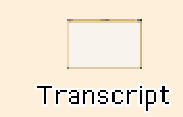
\includegraphics{TranscriptThumbnail}\hfill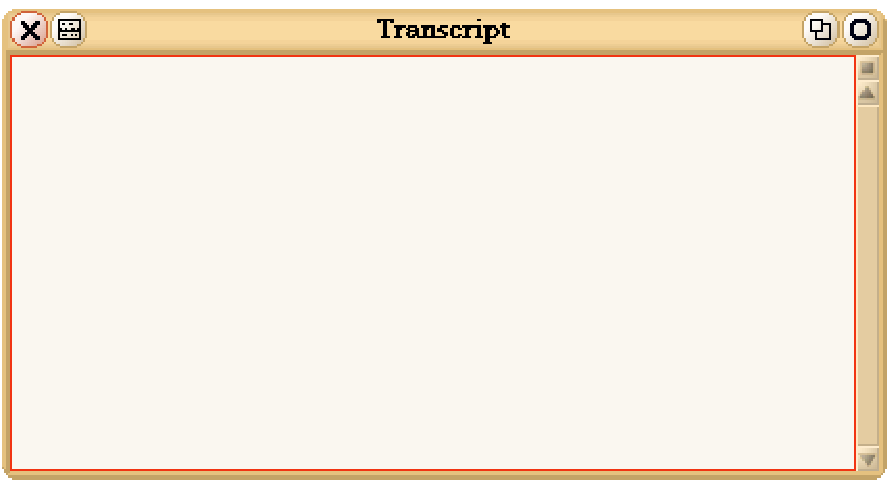
\includegraphics[width=8cm]{Transcript}
\caption{To bring a transcript drag and drop the thumbnail that you can find in a flap.}
\label{fig:transcript}
\end{center}
\end{figure}

To display information on the transcript there are two main messages \ct{show:} and \ct{cr}. The message \ct{show: aString} displays the string in the transcript and the message \ct{cr} inserts a new line in the transcript.    

\begin{scriptwithtitle}{Displaying information into a Transcript}\label{scr:transcript}
Transcript show: 'squeak is cool'.
Transcript cr.
Transcript show: 'really cool'
\end{scriptwithtitle}

\begin{figure}[h]
\begin{center}
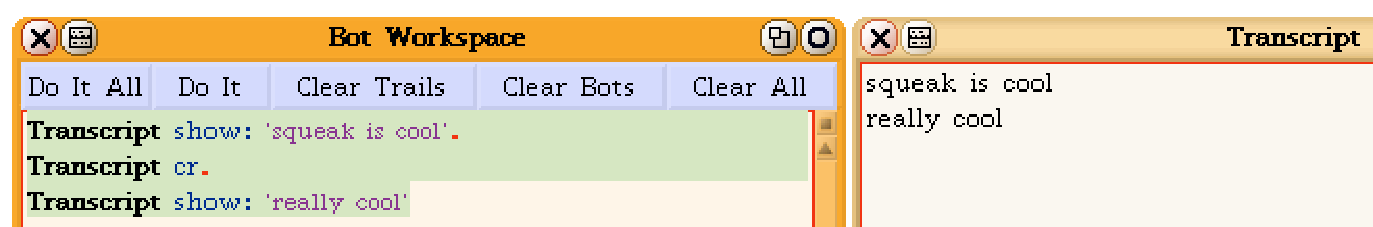
\includegraphics[width=\linewidth]{TranscriptCool.pdf}
\caption{Writing to the transcript.}
\end{center}
\end{figure}

Note that the Transcript only displays strings. Therefore when we want to display a number we have to obtain a string representing it using the method \ct{asString} as shown by \scrref{src:transcriptNumber}.

\begin{scriptwithtitle}{Converting a number in a string before displaying it}\label{src:transcriptNumber}
Transcript show: '21 + 21 is: ', 42 asString ; cr

| answerNumber |
answerNumber := 42.
Transcript show: '21 + 21 is: ', answerNumber asString.
\end{scriptwithtitle}


\section{Generating and Understanding a Trace}
Now we would like to show you how we can use the Transcript to generate a trace of a program. A trace is a collection of indications that is generated by a program. 
To generate a trace, we introduce expressions that do not change the original execution of the program but for example display information to the transcript. Let us experiment with script~\ref{src:strangestairhere} that draws a stair with steps of growing length.

\begin{scriptwithtitle}{Stairs}\label{src:strangestairhere}
| \caro length |
\caro := \Turtle new.
length := 10.
10 timesRepeat: 
                [ \caro go: length.
                \caro turnLeft: 90.
                \caro go: 5.
                \caro turnRight: 90.
                length := length + 10 ]
\end{scriptwithtitle}

The first simple trace that we can generate is to introduce expression that display an information before and after the loop as shown in \scrref{src:strangestairhere2}.

\begin{scriptwithtitle}{Stairs}\label{src:strangestairhere2}
| \caro length |
\caro := \Turtle new.
length := 10.
\textbf{Transcript show: 'Before the loop' ; cr.}
10 timesRepeat: 
                [ \caro go: length.
                \caro turnLeft: 90.
                \caro go: 5.
                \caro turnRight: 90.
                length := length + 10 ].
\textbf{Transcript show: 'After the loop' ; cr.}
\end{scriptwithtitle}

Modify the previous program and introduce the expression \ct{Transcript show: 'inside the loop' ; cr.} inside the loop. You should get 10 times the 'inside the loop' information on the transcript.  You can also insert the expression \ct{self halt} to get a debugger.



Now we would like to  use the same technique to generate a more sophisticated trace. For example, we want to see how the value of the variable \ct{length} evolves while the program is executed. The following script~\ref{scr:traceOne} contains a new expression that prints the value of the variable \ct{length} at the beginning of the loops each time it is  executed.

\begin{scriptwithtitle}{Stairs}\label{src:strangestairtrace}\label{scr:traceOne}
| \caro length |
\caro := \Turtle new.
length := 10.
10 timesRepeat: 
                [ \bold{Transcript show: '>> ',  length asString ; cr.}
                \caro go: length.
                \caro turnLeft: 90.
                \caro go: 5.
                \caro turnRight: 90.
                length := length + 10 ]
\end{scriptwithtitle}


\begin{figure}
\begin{center}
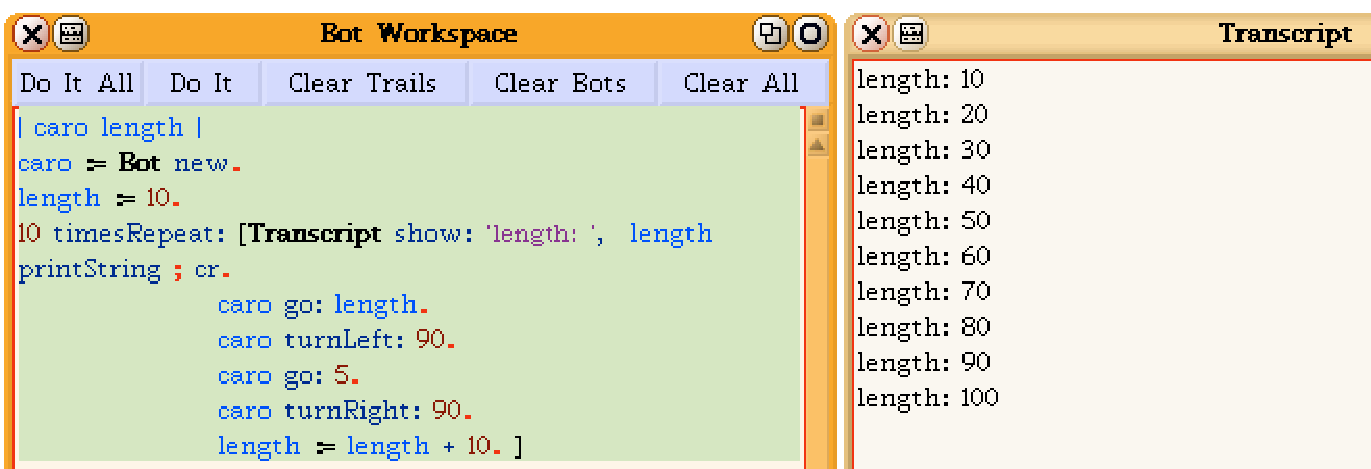
\includegraphics[width=\linewidth]{Stairs}
\caption{Adding a trace to a script. }
\end{center}
\end{figure}


Adding a trace after assignments is often interesting and reveals some key behavior of a porgram. For example, we suggest you to add the expression \ct{Transcript show: 'After := ' , length asString ;cr.} after the last expression of the loop as in the script~\ref{src:strangestairtrace2}. The trace shows the value of the variable \ct{length} at the beginning and the end of the loop. 

\begin{scriptwithtitle}{Stairs}\label{src:strangestairtrace2}
\begin{tabbing}
aaaaaaaaaaaaaaaaaaaaaaaaaaaaaaaaaaaaaaaaaaaaaaaaaaaaaaaaaaaaaaaaa\=aaaaaaaaaaaaaaaaaaaaaaaa=\kill
| \caro length | \> length: 10\\
\caro := \Turtle new.\> length after := 20\\
length := 10.\> length: 20 \\
10 timesRepeat: [ Transcript show: 'length: ',  length asString ; cr. \> length after := 30\\
                \caro go: length. \> length: 30 \\
                \caro turnLeft: 90. \> length after := 40\\
                \caro go: 5. \> length: 40\\
                \caro turnRight: 90. \> length after := 50\\
                length := length + 10. \> length: 60 \\
                \bold{Transcript show: ' length after := ' , length asString ; cr.} ] \> length after := 60\\
                \> length: 70\\
                \> length after := 70 \\
                \> length: 80\\
                \> length after := 90\\
                \> length: 90\\
                \> length after := 100\\
                \> length: 100\\
                \> length after := 110
\end{tabbing}
\end{scriptwithtitle}


\summa



\begin{itemize}
\item A string is a sequence of characters delimited by  single quotes \ct{'}. A string  represent textual information such as words or sentences and is used to display information to the user. \ct{'squeak is cool'} is a string of 14 characters. 

\item A character is one letter prefixed by the dollar sign \ct{\$}. \ct{\$a} is the character a.

\item A string can represent a number but this is not a number. For example, the string \ct{'69'} is composed of the two characters: \ct{\$6} and \ct{\$9}. To obtain the string representing a number, send the message \ct{asString} to it.

\item The Transcript is a small window used to display message for the user. 
The message \ct{show: aString} displays the argument into the Transcript. The message \ct{cr} adds a new line in the Transcript. 
\end{itemize}

\ifx\wholebook\relax\else
\end{document}\fi
